\documentclass[12pt]{article}
\usepackage{amsmath,amssymb}
\usepackage{geometry}
\geometry{margin=1in}
\usepackage{tikz}
\usetikzlibrary{decorations.pathreplacing,arrows.meta}
\usepackage{caption}
\usepackage{hyperref}

\title{Exact Analytical Solution of the Viscous Burgers' Equation via the Cole--Hopf Transformation}
\author{}
\date{}

\begin{document}
\maketitle

\section*{Introduction}



This report presents the derivation of the exact analytical solution to the one-dimensional viscous Burgers' equation with Riemann step initial data under Dirichlet boundary conditions representing a shock tube setup. Through the Cole--Hopf transformation, the nonlinear PDE is linearized to the heat equation, enabling explicit construction of the solution. The resulting travelling viscous shock wave solution is given in closed form by a hyperbolic tangent profile, providing a canonical benchmark for numerical analysis and theoretical study.

\vspace{12pt}

\section*{1. Problem Statement}

We consider a one-dimensional shock tube of length L, initially partitioned into two regions by an imaginary membrane.The tube contains a scalar compressible fluid velocity field u(x,t), governed by the viscous Burgers equation:

\begin{equation}
\label{eq:burgers}
\frac{\partial u}{\partial t} + u \frac{\partial u}{\partial x} = \nu \frac{\partial^2 u}{\partial x^2},
\end{equation}
defined on the spatial interval \(x \in [0,1]\) for time \(t > 0\), where \(u(x,t)\) is the velocity field and \(\nu > 0\) is the kinematic viscosity.

The initial velocity profile is the Riemann step:
\[
u(x,0) = \begin{cases}
1, & x \le 0.5, \\[6pt]
0, & x > 0.5,
\end{cases}
\]
with fixed boundary conditions for all \(t>0\):
\[
u(0,t) = 1, \quad u(1,t) = 0.
\]

\vspace{12pt}

Wave Phenomena: When the diaphragm is removed, the pressure difference drives the fluid.
This creates a shock wave that propagates into the lower-pressure region, and a rarefaction
wave that propagates into the higher-pressure region. A contact discontinuity also forms
between the two regions, separating the two fluids.
The contact discontinuity is a region where density and entropy can change, but pressure
and the normal component of velocity are constant across it.

\vspace{12pt}

\noindent\textbf{Shock Tube Illustration:}

\begin{center}
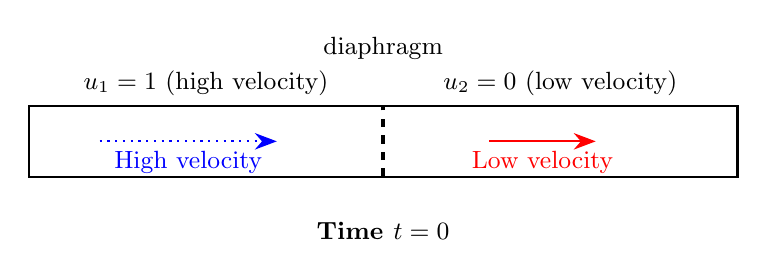
\begin{tikzpicture}[scale=0.9, every node/.style={font=\small}]
  % Tube at initial time
  \draw[thick] (0,0) rectangle (10,1);
  \draw[ultra thick, dashed] (5,0) -- (5,1) node[midway, above=9mm] {diaphragm};

  \node[above] at (2.5,1) {$u_1 = 1$ (high velocity)};
  \node[above] at (7.5,1) {$u_2 = 0$ (low velocity)};

  % Blue dotted velocity arrow (initial high velocity)
  \draw[-{Stealth[scale=1.2]}, thick, blue, dotted] (1,0.5) -- (3.5,0.5);

  % Red solid velocity arrow (low velocity)
  \draw[-{Stealth[scale=1.2]}, thick, red] (6.5,0.5) -- (8,0.5);

  \node[blue] at (2.25,0.2) {High velocity};
  \node[red] at (7.25,0.2) {Low velocity};
  
  \node[below] at (5,-0.5) {\textbf{Time \(t=0\)}};
\end{tikzpicture}
\end{center}

\vspace{12pt}

\begin{center}
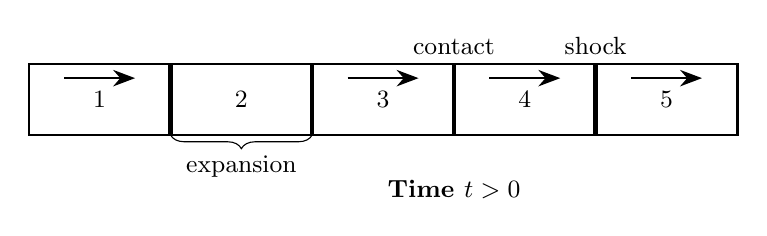
\begin{tikzpicture}[scale=0.9, every node/.style={font=\small}]
  % Tube at later time t > 0
  \draw[thick] (0,0) rectangle (10,1);

  % Expansion region boundaries
  \draw[ultra thick] (2,0) -- (2,1);
  \draw[ultra thick] (4,0) -- (4,1);

  % Contact discontinuity and shock wave
  \draw[ultra thick] (6,0) -- (6,1);
  \draw[ultra thick] (8,0) -- (8,1);

  % Subregion labels
  \node at (1,0.5) {1};
  \node at (3,0.5) {2};
  \node at (5,0.5) {3};
  \node at (7,0.5) {4};
  \node at (9,0.5) {5};

  % Brace marking expansion zone
  \draw[decorate, decoration={brace, amplitude=5pt, mirror}] (2,0) -- (4,0)
    node[midway, below=4pt] {expansion};

  \node[above] at (6,1) {contact};
  \node[above] at (8,1) {shock};

  % Velocity arrows indicating flow directions
  \draw[-{Stealth[scale=1.2]}, thick] (0.5,0.8) -- (1.5,0.8);
  \draw[-{Stealth[scale=1.2]}, thick] (4.5,0.8) -- (5.5,0.8);
  \draw[-{Stealth[scale=1.2]}, thick] (6.5,0.8) -- (7.5,0.8);
  \draw[-{Stealth[scale=1.2]}, thick] (8.5,0.8) -- (9.5,0.8);

  \node[below] at (6,-0.5) {\textbf{Time \(t > 0\)}};
\end{tikzpicture}
\end{center}

\vspace{20pt}

\section*{2. Cole--Hopf Transformation and Linearization}

To solve \eqref{eq:burgers}, we apply the Cole--Hopf transformation,
\[
u(x,t) = - 2 \nu \frac{\partial_x \varphi(x,t)}{\varphi(x,t)},
\]
which transforms the nonlinear equation into the linear heat equation for \(\varphi(x,t)\):
\[
\frac{\partial \varphi}{\partial t} = \nu \frac{\partial^2 \varphi}{\partial x^2}.
\]

The initial condition for \(\varphi\) is derived by integrating
\[
\frac{\partial_x \varphi(x,0)}{\varphi(x,0)} = -\frac{u(x,0)}{2 \nu}.
\]
Explicit integration yields
\[
\varphi_0(x) := \varphi(x,0) = A \exp\left(- \frac{1}{2 \nu} \int_0^x u(s,0) ds \right),
\]
where \(A\) is an arbitrary nonzero constant.

For the Riemann step initial data,
\[
\int_0^x u(s, 0) ds = \begin{cases}
x, & x \le 0.5, \\[6pt]
0.5, & x > 0.5,
\end{cases}
\quad \Rightarrow \quad
\varphi_0(x) = \begin{cases}
A e^{-x/(2 \nu)}, & x \le 0.5, \\[6pt]
A e^{-0.5/(2 \nu)}, & x > 0.5.
\end{cases}
\]

\vspace{20pt}

\section*{3. Travelling Viscous Shock Wave Solution:}

Assuming a travelling wave solution of the form
\[
u(x,t) = U(z), \quad z := x - c t,
\]
the PDE reduces to
\[
- c U' + U U' = \nu U'',
\]
where the prime denotes \(d/dz\).

Integrating once,
\[
\nu U' = \frac{U^2}{2} - c U + K,
\]
with constant of integration \(K\).

Boundary conditions require
\[
\lim_{z \to -\infty} U(z) = u_L = 1, \quad \lim_{z \to +\infty} U(z) = u_R = 0,
\]
implying \(U'\to 0\) at boundaries, hence
\[
\frac{u_L^2}{2} - c u_L + K = 0, \quad \frac{u_R^2}{2} - c u_R + K = 0.
\]
Subtracting yields
\[
c = \frac{u_L + u_R}{2} = \frac{1}{2}.
\]
Plugging back,
\[
K = \frac{1}{2} u_L^2 - c u_L = \frac{1}{2} - \frac{1}{2} = 0.
\]

Rearranged ODE:
\[
\nu \frac{dU}{dz} = \frac{1}{2} (U - u_L)(U - u_R) = \frac{1}{2} U (U - 1).
\]

Separate and integrate:
\[
\int \frac{dU}{U(U - 1)} = \int \frac{dz}{2 \nu}.
\]
Partial fractions yield
\[
\frac{1}{U(U-1)} = -\frac{1}{U} + \frac{1}{U - 1}.
\]

Integrating,
\[
- \ln|U| + \ln|U - 1| = \frac{z}{2 \nu} + C,
\]
or
\[
\ln\left| \frac{U - 1}{U} \right| = \frac{z}{2 \nu} + C.
\]
Exponentiating,
\[
\frac{U - 1}{U} = C_1 e^{z/(2 \nu)}.
\]

Choosing \(C_1\) to fix shock position at \(x_0\), solve for \(U(z)\):
\[
U(z) = \frac{1}{1 - C_1 e^{z/(2 \nu)}}.
\]

Equivalent and more illuminating form is
\[
\boxed{
u(x,t) = \frac{1}{2} - \frac{1}{2} \tanh\left( \frac{1}{4 \nu} \left( x - x_0 - \frac{1}{2} t \right) \right),
}
\]
characterizing a smooth viscous shock travelling at speed \(0.5\).

\vspace{20pt}

\section*{4. Physical Interpretation}

\begin{itemize}
  \item The solution describes a shock wave moving rightwards at speed \(c=0.5\), transitioning smoothly from velocity \(1\) on the left to zero on the right.
  \item The shock thickness scales with viscosity \(\nu\) as \(\delta \sim 4 \nu\).
  \item As \(\nu \to 0\), the solution approaches the inviscid discontinuous step.
  \item The Cole--Hopf transform potential \(\varphi\) corresponds to a scaled hyperbolic cosine profile.
\end{itemize}

\vspace{20pt}

\section*{5. Summary}

The viscous Burgers' equation with step initial and Dirichlet boundary conditions admits an explicit exact travelling wave solution via the Cole--Hopf transformation. The shock travels at the average of left and right velocities, with smooth thickness controlled by the viscosity. This exact solution serves as the definitive analytic benchmark for numerical simulations of viscous shocks within a finite domain.

\vspace{20pt}

\end{document}
